%% img/Reducibility.tex
%% Copyright 2019 Andrea Berlingieri
%
% This work may be distributed and/or modified under the
% conditions of the LaTeX Project Public License, either version 1.3
% of this license or (at your option) any later version.
% The latest version of this license is in
%   http://www.latex-project.org/lppl.txt
% and version 1.3 or later is part of all distributions of LaTeX
% version 2005/12/01 or later.
%
% This work has the LPPL maintenance status `maintained'.
%
% The Current Maintainer of this work is Andrea Berlingieri.
%
% This work consists of all files listed in manifest.txt
\documentclass{standalone}

\usepackage{TikzStyle}
\usepackage{mystyle}

\begin{document}
    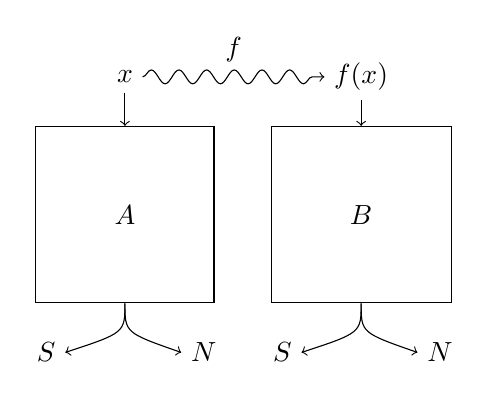
\begin{tikzpicture}
        \node (x) at (1,0) {$x$};
        \node (fx) at (4,0) {$f(x)$};
        \draw [->,decorate,decoration=snake] (x) -- (fx) node [pos=0.5,yshift=10pt] {$f$};
        \node[draw,inner sep=1cm] (A) at (1,-1.75) {$A$};
        \node[draw,inner sep=1cm] (B) at (4,-1.75) {$B$};
        \draw [->] (x) -- (A);
        \draw [->] (fx) -- (B);
        \node (s1) at (0,-3.5) {$S$};
        \node (n1) at (2,-3.5) {$N$};
        \node (s2) at (3,-3.5) {$S$};
        \node (n2) at (5,-3.5) {$N$};
        \draw [->] (A.south) .. controls (1,-3.25) and (1,-3.25) .. (s1.east);
        \draw [->] (A.south) .. controls (1,-3.25) and (1,-3.25) .. (n1.west);
        \draw [->] (B.south) .. controls (4,-3.25) and (4,-3.25) .. (s2.east);
        \draw [->] (B.south) .. controls (4,-3.25) and (4,-3.25) .. (n2.west);
    \end{tikzpicture}
\end{document}
